% !TEX program = xelatex
\documentclass[12pt,a4paper]{article}
\usepackage[a4paper,margin=2.5cm]{geometry}
\usepackage{fontspec}
\usepackage[main=vietnamese,english]{babel}
\usepackage{graphicx}
\usepackage{booktabs}
\usepackage{tabularx}
\usepackage{array}
\usepackage{makecell}
\usepackage{float}
\usepackage{caption}
\usepackage{subcaption}
\usepackage{amsmath}
\usepackage{xcolor}
\usepackage{hyperref}
\usepackage{url}

\setmainfont{TeX Gyre Termes}
\setsansfont{TeX Gyre Heros}
\setmonofont{DejaVu Sans Mono}

\addto\captionsvietnamese{
  \renewcommand{\contentsname}{Mục lục}
  \renewcommand{\tablename}{Bảng}
  \renewcommand{\figurename}{Hình}
  \renewcommand{\refname}{Tài liệu tham khảo}
  \renewcommand{\appendixname}{Phụ lục}
}

\newcommand{\codesize}{\footnotesize}
\newcommand{\tablecodesize}{\scriptsize}
\newcommand{\model}[1]{\texttt{\small\detokenize{#1}}}
\newcommand{\algo}[1]{\textsc{#1}}
\newcommand{\metric}[1]{\textit{#1}}
\newcommand{\tablemodel}[1]{%
  \begingroup
  \tablecodesize\ttfamily
  \Urlmuskip=0mu plus 2mu\relax
  \nolinkurl{#1}%
  \endgroup
}
\newcolumntype{Y}{>{\raggedright\arraybackslash}X}
\newcolumntype{L}[1]{>{\raggedright\arraybackslash}p{#1}}

\hypersetup{colorlinks=true,linkcolor=blue,citecolor=blue,urlcolor=blue}
\graphicspath{{figures/}}
\captionsetup{font=small,labelfont=bf}

\begin{document}
\begin{titlepage}
\centering

\includegraphics[width=0.18\linewidth]{hust.jpg}\par\vspace{1cm}
{\Large Trường Đại học Bách khoa Hà Nội\par}
{\large Project II\par}
\vspace{1.5cm}
{\LARGE \textbf{Đánh giá so sánh các thuật toán phân cụm trên không gian vector đa đặc trưng cho dữ liệu tin tức tài chính}\par}
\vspace{1.2cm}
\begin{tabular}{ll}
\textbf{Sinh viên:} & [Tên sinh viên]\\
\textbf{Mã số sinh viên:} & [MSSV]\\
\textbf{Lớp/Chương trình:} & [Lớp/Chương trình đào tạo]\\
\textbf{Giảng viên hướng dẫn:} & [Tên giảng viên]\\
\end{tabular}
\vfill
{\large Hà Nội, 2026\par}
\end{titlepage}

\tableofcontents
\section{Giới thiệu}

Dữ liệu tin tức tài chính là một nguồn thông tin khó phân tích do khối lượng lớn, nội dung ngắn, và nhiều tín hiệu nhiễu từ nguồn phát hành, mã cổ phiếu hoặc thời gian. Đồ án này đánh giá các thuật toán phân cụm trên không gian vector văn bản và vector đa đặc trưng, hướng tới hai vai trò: phân cụm phủ toàn bộ dữ liệu (full-coverage clustering) và phát hiện cụm dày hoặc cụm dạng sự kiện (dense/event detection).

Mục tiêu chính là so sánh \algo{MiniBatchKMeans}, \algo{Gaussian Mixture Model}, \algo{HDBSCAN} và \algo{CLARA} theo các chỉ số nội tại như \metric{silhouette}, \metric{Davies-Bouldin Index} (DBI), độ phủ, độ ổn định ARI/NMI, cân bằng kích thước cụm và hậu kiểm metadata. Báo cáo không chọn mô hình chỉ bằng một metric đơn lẻ, mà xem xét vai trò sử dụng của từng nhóm thuật toán.

\section{Cơ sở lý thuyết và nghiên cứu liên quan}

Phân cụm văn bản tài chính thường dựa trên biểu diễn embedding để chuyển các headline ngắn thành vector số. Các thuật toán centroid-based như \algo{MiniBatchKMeans} phù hợp khi cần gán nhãn cho toàn bộ dữ liệu và kiểm soát số cụm. Các mô hình xác suất như \algo{GMM} cung cấp một baseline khác dựa trên phân phối, trong khi \algo{HDBSCAN} phù hợp hơn với việc phát hiện các vùng dày đặc và cho phép một phần điểm dữ liệu được xem là nhiễu.

Trong bối cảnh dữ liệu tin tức, trực quan hóa \algo{PCA} hoặc \algo{UMAP} chỉ nên được xem là công cụ chẩn đoán. Cấu trúc cụm trong không gian 2D/3D có thể khác đáng kể so với không gian embedding nhiều chiều, nên quyết định mô hình cần dựa trên các metric định lượng và kiểm tra diễn giải.

\section{Dữ liệu}

Dữ liệu đầu vào gồm các headline và thông tin liên quan đến tin tức tài chính. Pipeline tiền xử lý chuẩn hóa văn bản, loại bỏ nhiễu cơ bản và tạo các trường phục vụ phân tích. Các embedding văn bản được kết hợp với một số đặc trưng phụ dạng bảng như đặc trưng lexical, lịch, publisher, stock và tín hiệu sentiment/risk trong các thí nghiệm mở rộng.

Phiên bản báo cáo hiện tại tập trung vào tập 100k dòng đã được dùng cho các thí nghiệm cuối. Các artifact lớn như embedding `.npy` và label CSV kích thước lớn không được đưa trực tiếp vào project LaTeX.

\section{Phương pháp thực hiện}

Pipeline thực nghiệm gồm các bước: tiền xử lý dữ liệu, sinh embedding, xây dựng không gian đặc trưng, chạy thuật toán phân cụm, tính metric, hậu kiểm metadata và tổng hợp báo cáo. Các không gian đặc trưng chính gồm embedding gốc 768 chiều, PCA64 của embedding, và các biến thể có thêm đặc trưng lexical hoặc metadata có trọng số.

Các thuật toán được đánh giá theo hai vai trò. Với full-coverage clustering, mô hình cần gán cụm cho toàn bộ dữ liệu và giữ cân bằng kích thước cụm hợp lý. Với event/dense detection, \algo{HDBSCAN} được đánh giá theo chất lượng cụm dày, coverage, noise ratio và negative silhouette thay vì yêu cầu coverage 100\%.

\section{Thiết kế thực nghiệm}

Các thực nghiệm được tổ chức theo từng nhóm để giữ phạm vi đánh giá rõ ràng và tránh sweep quá rộng sau giai đoạn tuning chính:

\begin{itemize}
  \item MiniBatch k-sweep trên các không gian biểu diễn chính để chọn baseline và ứng viên full-coverage.
  \item Representation tuning để kiểm tra tác động của PCA, L2 normalization và đặc trưng lexical.
  \item Bounded multi-feature ablation để đánh giá tác động của các đặc trưng phụ như calendar, publisher, stock và lexicon.
  \item Compact HDBSCAN tuning cho vai trò phát hiện cụm dày hoặc sự kiện, không thay thế mô hình full-coverage.
  \item CLARA true và GMM để tạo baseline/diagnostic reference cho các họ thuật toán khác.
\end{itemize}

Các metric chính gồm \metric{silhouette}, \metric{DBI}, coverage, noise ratio, negative silhouette, cluster balance, stability ARI/NMI và các cảnh báo metadata dominance.

\section{Kết quả thực nghiệm}

Bảng~\ref{tab:final-models} tóm tắt các quyết định cuối cùng. Các mô hình được phân vai như sau:

\begin{itemize}
  \item Conservative full-coverage baseline: \model{text_768_original + minibatch_k16}.
  \item Best experimental full-coverage model: \model{text_pca64_lexical + minibatch_k40}.
  \item Event/dense detection model: \model{text_pca64_only + HDBSCAN(min_cluster_size=30, min_samples=20, cluster_selection_method=leaf)}.
  \item High-silhouette risky reference: \model{text_pca64_only + minibatch_k96}, chỉ dùng để tham chiếu về rủi ro phân mảnh.
\end{itemize}

\begin{table}[H]
\centering
\small
\caption{So sánh rút gọn các mô hình cuối cùng.}
\label{tab:final-models}
\begin{tabularx}{\textwidth}{L{0.24\textwidth} L{0.32\textwidth} r r r r Y}
\toprule
Vai trò & Mô hình & Coverage (\%) & Số cụm & Silhouette & DBI & Ghi chú \\
\midrule
Conservative baseline & \tablemodel{text_768_original + minibatch_k16} & 100.00 & 16 & 0.0632 & 3.0854 & Full-coverage, số cụm vừa phải, dùng làm baseline thận trọng. \\
Selected experimental & \tablemodel{text_pca64_lexical + minibatch_k40} & 100.00 & 40 & 0.1065 & 3.3463 & Cân bằng tốt giữa metric, kích thước cụm và khả năng diễn giải. \\
Event detection & \tablemodel{text_pca64_only + HDBSCAN(mcs=30, ms=20, leaf)} & 20.12 & 219 & 0.6086 & 1.0260 & Phát hiện cụm dày; không nhắm coverage 100\%. \\
Risk reference & \tablemodel{text_pca64_only + minibatch_k96} & 100.00 & 96 & 0.1161 & 2.9968 & Metric mạnh nhưng rủi ro phân mảnh và metadata warning cao. \\
\bottomrule
\end{tabularx}
\end{table}

\begin{table}[H]
\centering
\scriptsize
\caption{Kiểm chứng HDBSCAN cho phát hiện cụm dày/sự kiện.}
\label{tab:hdbscan-event-validation}
\begin{tabularx}{\textwidth}{L{0.28\textwidth} r r r r r r r Y}
\toprule
Cấu hình & Fit rows & Coverage & Noise & Số cụm & Sil. cos & DBI & Neg. sil. & Ghi chú \\
\midrule
\tablemodel{text_pca64_only, mcs=30, ms=20, leaf} & 100000 & 20.12 & 79.88 & 219 & 0.6086 & 1.0260 & 0.69 & Selected event/dense detection model. \\
\tablemodel{text_768_original, hdbscan_minsize50} & 100000 & 20.64 & 79.36 & 105 & 0.5652 & 0.9861 & -- & Historical text-only baseline. \\
\tablemodel{text_pca64_only, mcs=50, eom} & 50000 & 23.20 & 76.80 & 28 & 0.2236 & 1.0837 & 55.09 & Same-sample PCA64 baseline, kém hơn rõ về silhouette. \\
\bottomrule
\end{tabularx}
\end{table}


\subsection{So sánh mở rộng giữa các thuật toán}

Bảng so sánh đầy đủ giữa các mô hình được chọn, các baseline và các cấu hình diagnostic/reference được trình bày trong Phụ lục, Bảng~\ref{tab:extended_algorithm_comparison}. Trong phần chính, báo cáo chỉ giữ lại các nhận xét tổng hợp và một số biểu đồ quan trọng để tránh làm nội dung quá tải.

% Extended algorithm comparison snippet for Overleaf.
\paragraph{So sánh mở rộng các thuật toán.}
Bảng~\ref{tab:extended_algorithm_comparison} tổng hợp thêm các mô hình không được chọn bên cạnh các mô hình cuối cùng. Mục tiêu của bảng không phải là xếp hạng mọi thuật toán bằng một metric duy nhất, mà là làm rõ vai trò của từng nhóm mô hình: full-coverage, event detection và diagnostic/reference. Với những metric không tương thích hoặc không có sẵn, bảng dùng ký hiệu ``--'' để tránh diễn giải quá mức.

\begin{itemize}
    \item \textbf{MiniBatchKMeans} là lựa chọn phù hợp nhất cho full-coverage vì gán cụm cho toàn bộ 100k điểm, chạy ổn định và có thể kiểm soát mức độ phân mảnh bằng tham số $k$. Baseline \texttt{text\_768\_original + minibatch\_k16} giữ vai trò thận trọng, còn \texttt{text\_pca64\_lexical + minibatch\_k40} là mô hình thực nghiệm được chọn nhờ cân bằng tốt hơn giữa silhouette, DBI và kích thước cụm.
    \item \textbf{GMM} là baseline xác suất có ích để đối chiếu với KMeans, nhưng không vượt rõ MiniBatchKMeans trên dữ liệu này. Vì vậy GMM được giữ làm mô hình tham chiếu thay vì mô hình chính.
    \item \textbf{HDBSCAN} không nhằm coverage 100\%, mà dùng để phát hiện cụm dày đặc hoặc cụm dạng sự kiện. Cấu hình \texttt{text\_pca64\_only + HDBSCAN(min\_cluster\_size=30, min\_samples=20, leaf)} được chọn vì silhouette cao, negative silhouette thấp và không có dấu hiệu collapse trong kiểm định full 100k.
    \item \textbf{CLARA} có giá trị như diagnostic baseline medoid-based. Tuy nhiên các kết quả CLARA true vẫn yếu hơn MiniBatchKMeans và chỉ chạy ở mức sample, nên không được chọn làm mô hình cuối cùng.
\end{itemize}

Tóm lại, MiniBatchKMeans được chọn cho nhánh full-coverage vì cân bằng tốt giữa độ phủ, chất lượng cụm và khả năng diễn giải. HDBSCAN được chọn riêng cho event detection vì nó phát hiện các vùng dày đặc thay vì cố gắng gán nhãn cho mọi điểm. GMM và CLARA đóng vai trò baseline/diagnostic, còn các cấu hình high-$k$ như \texttt{minibatch\_k96} chỉ nên xem là tham chiếu vì rủi ro phân mảnh và metadata dominance cao hơn.


\begin{figure}[H]
\centering
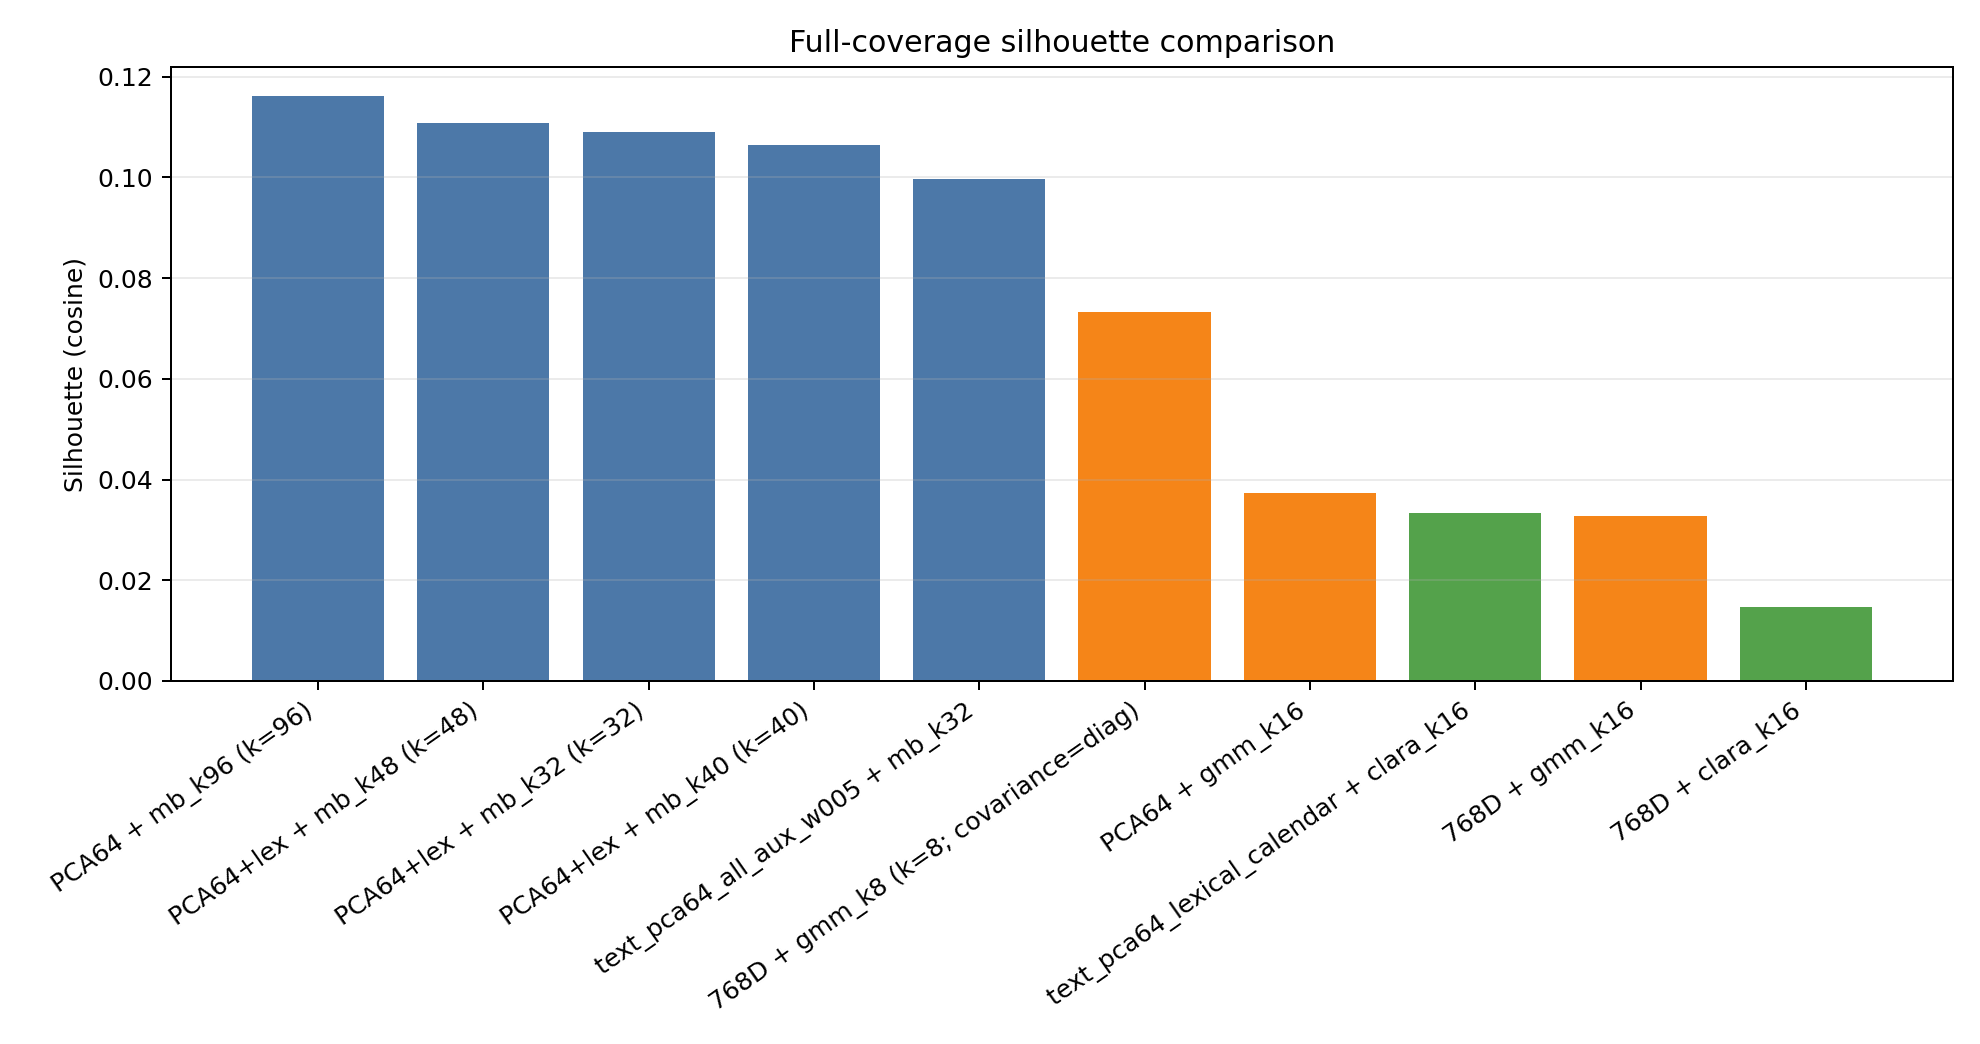
\includegraphics[width=0.82\linewidth]{full_coverage_silhouette_comparison.png}
\caption{So sánh \metric{silhouette} của các mô hình full-coverage và reference quan trọng.}
\label{fig:full-coverage-silhouette}
\end{figure}

\begin{figure}[H]
\centering
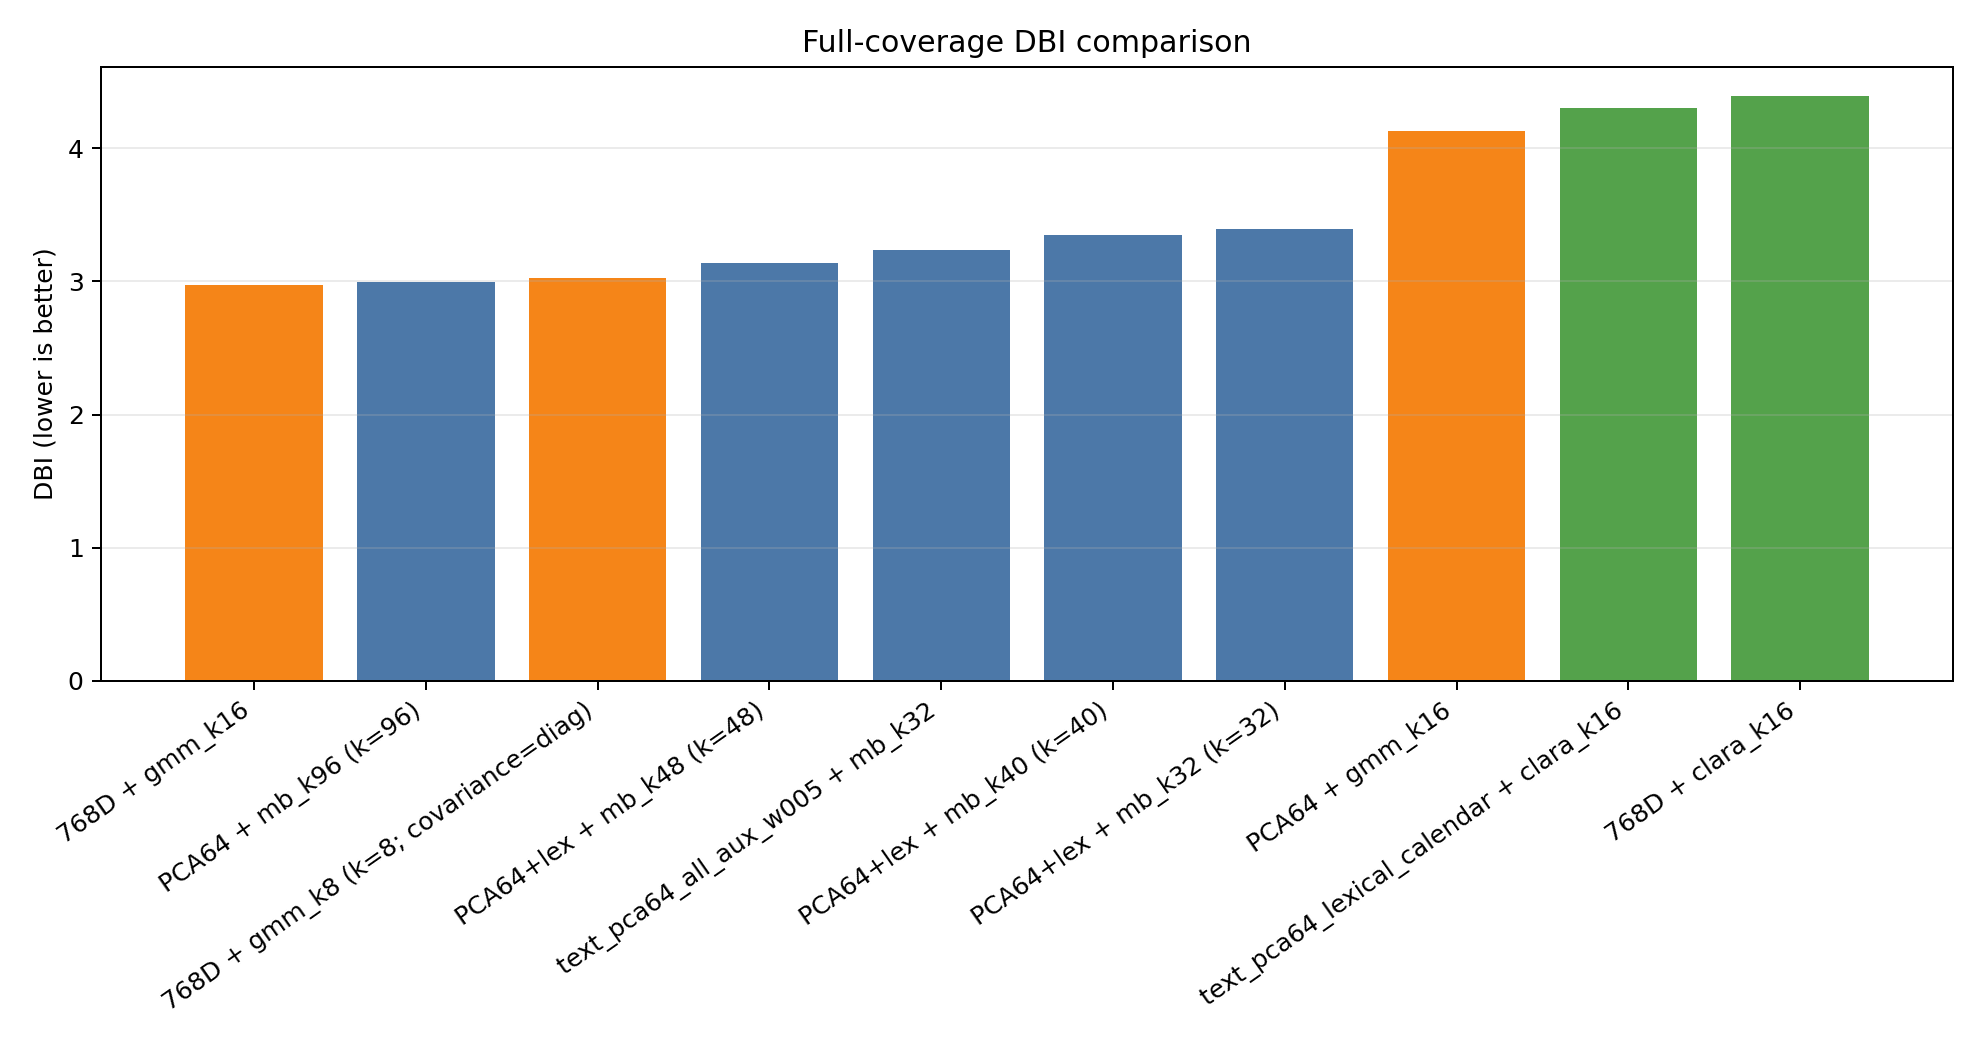
\includegraphics[width=0.82\linewidth]{full_coverage_dbi_comparison.png}
\caption{So sánh \metric{DBI} của các mô hình full-coverage và reference quan trọng.}
\label{fig:full-coverage-dbi}
\end{figure}

\begin{figure}[H]
\centering
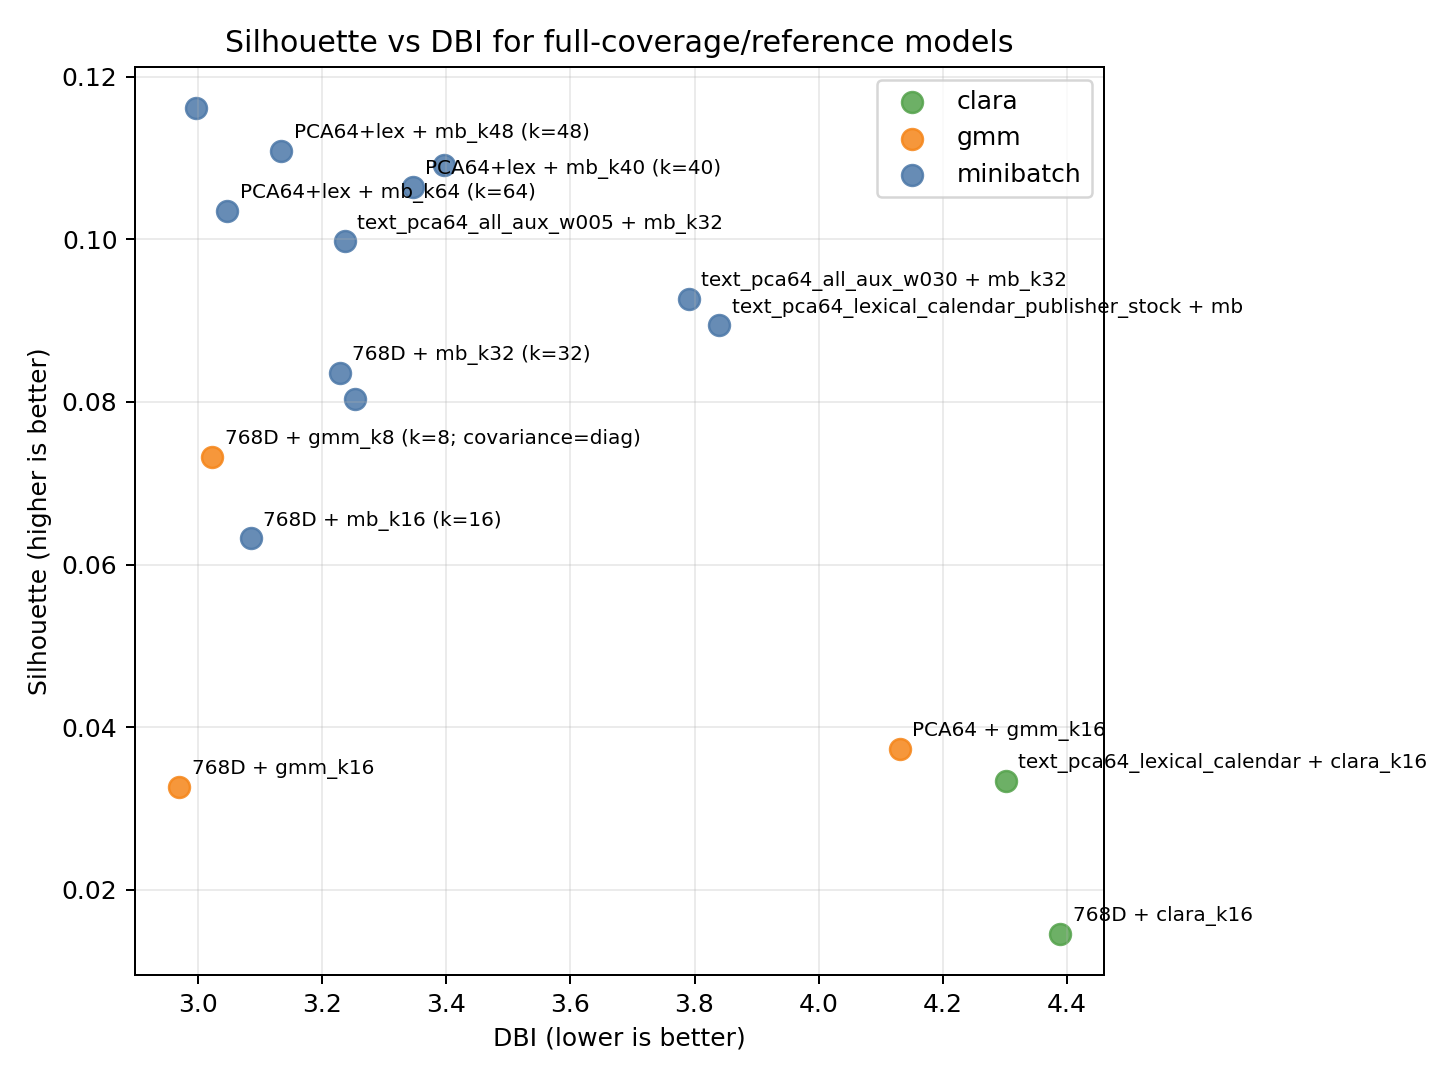
\includegraphics[width=0.78\linewidth]{model_scatter_silhouette_vs_dbi.png}
\caption{Quan hệ giữa \metric{silhouette} và \metric{DBI} theo family thuật toán.}
\label{fig:silhouette-dbi-scatter}
\end{figure}

\begin{figure}[H]
\centering
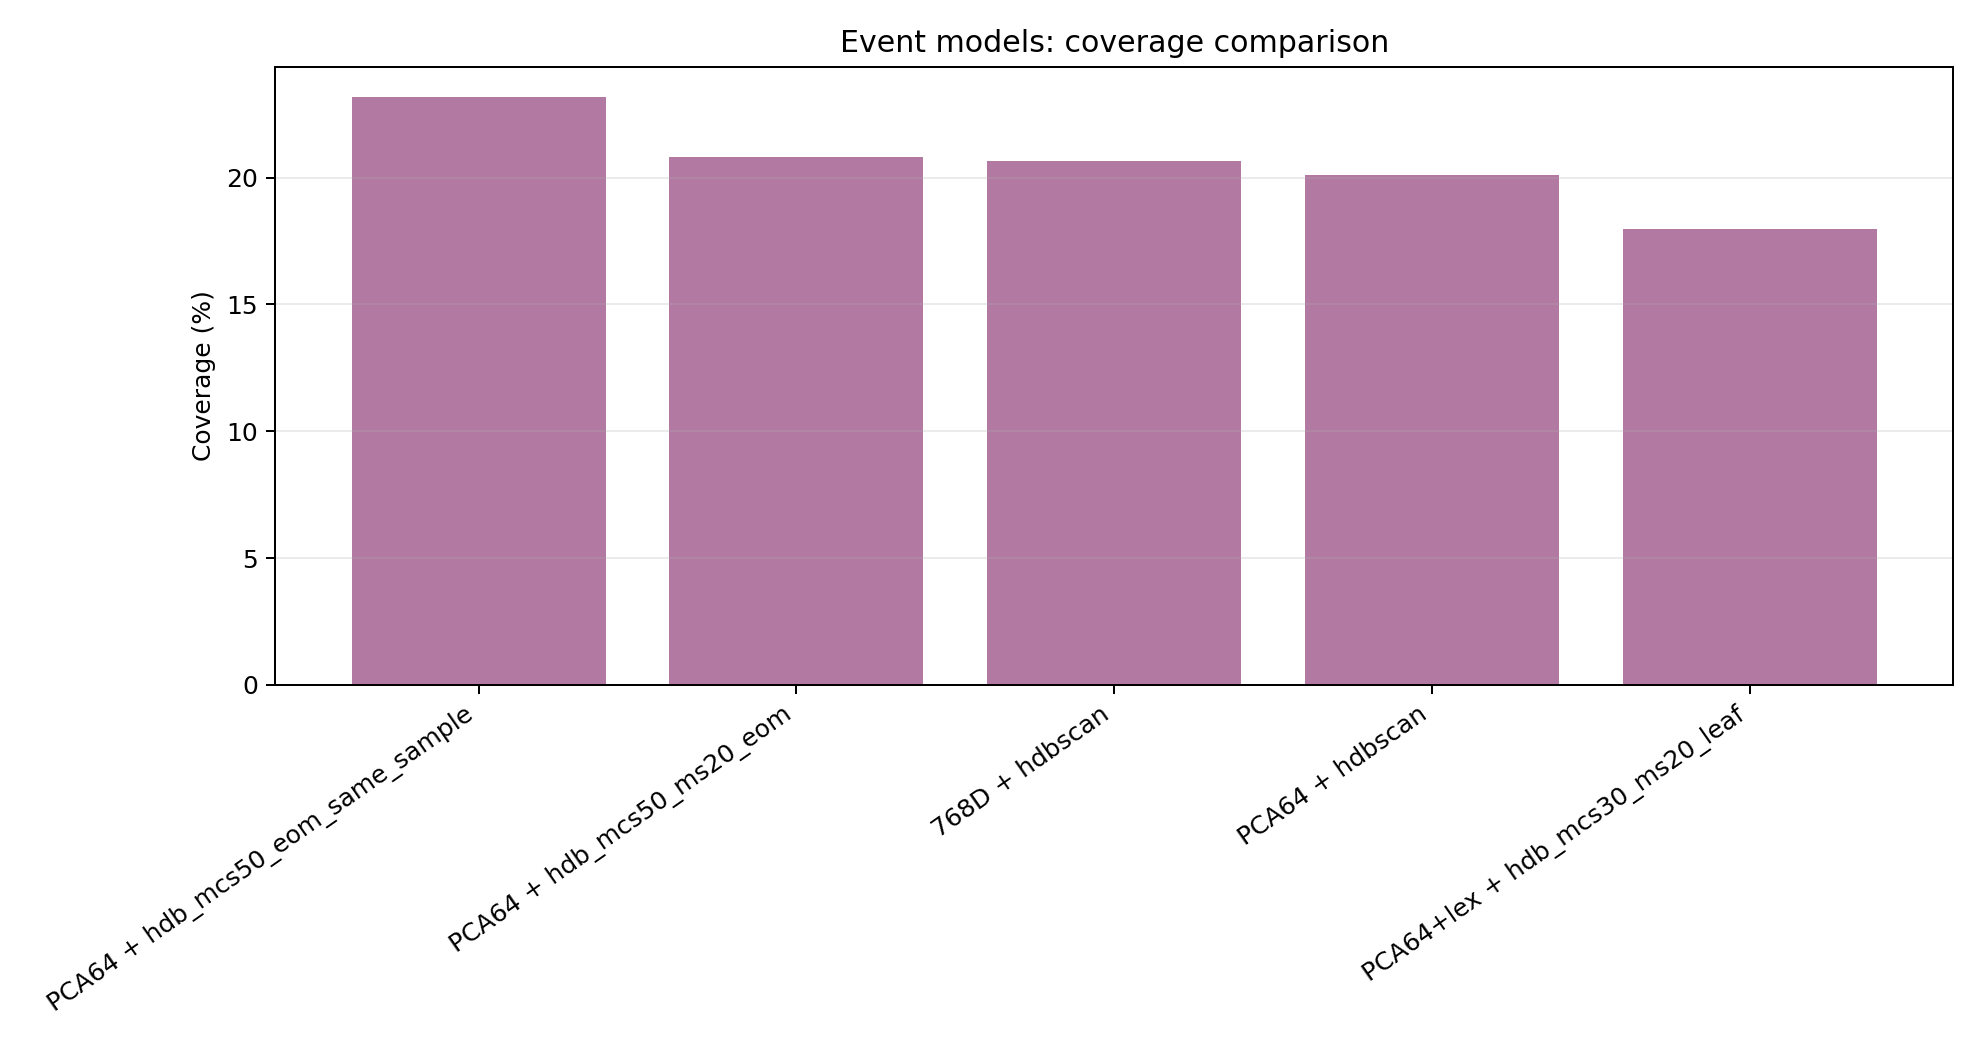
\includegraphics[width=0.82\linewidth]{event_models_coverage_comparison.png}
\caption{Coverage của các mô hình \algo{HDBSCAN} trong vai trò event/dense detection.}
\label{fig:event-coverage}
\end{figure}

\begin{figure}[H]
\centering
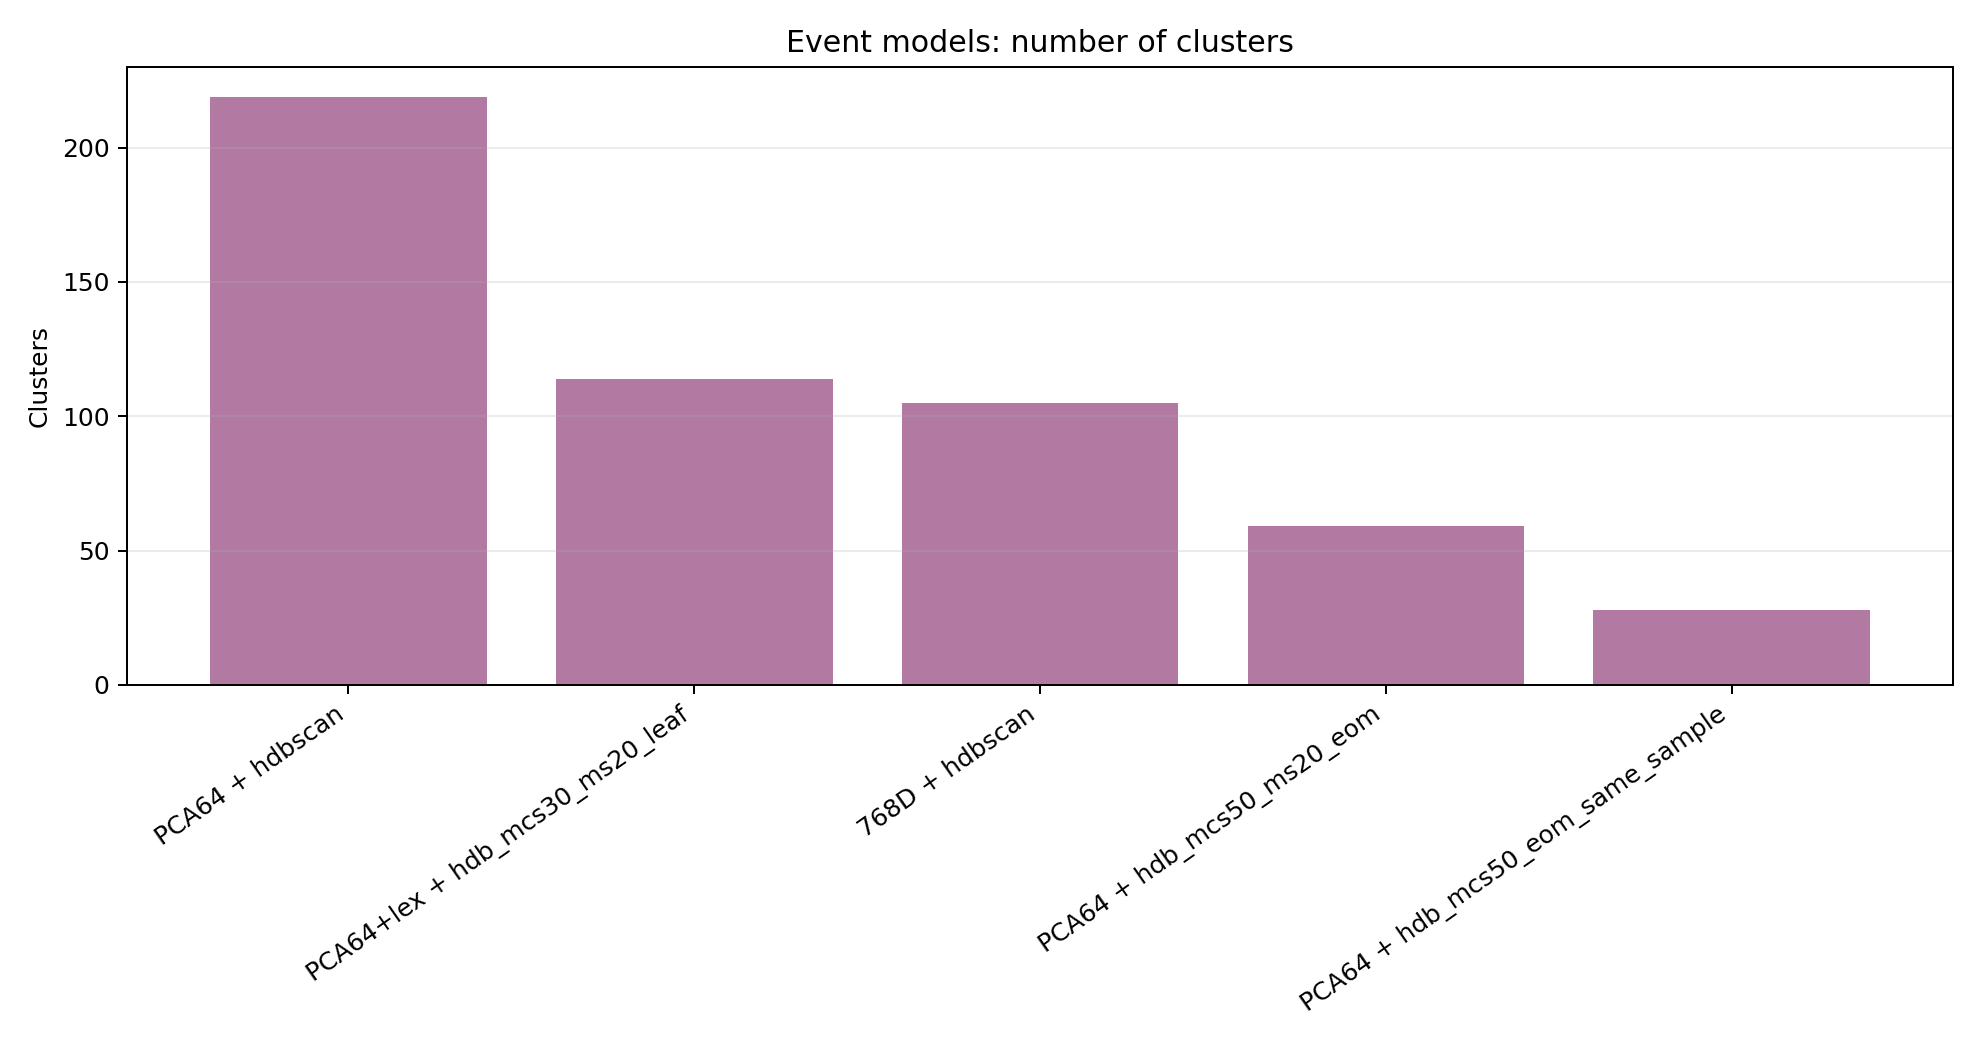
\includegraphics[width=0.82\linewidth]{event_models_cluster_count_comparison.png}
\caption{Số cụm của các mô hình \algo{HDBSCAN} trong vai trò event/dense detection.}
\label{fig:event-clusters}
\end{figure}

\begin{figure}[H]
\centering
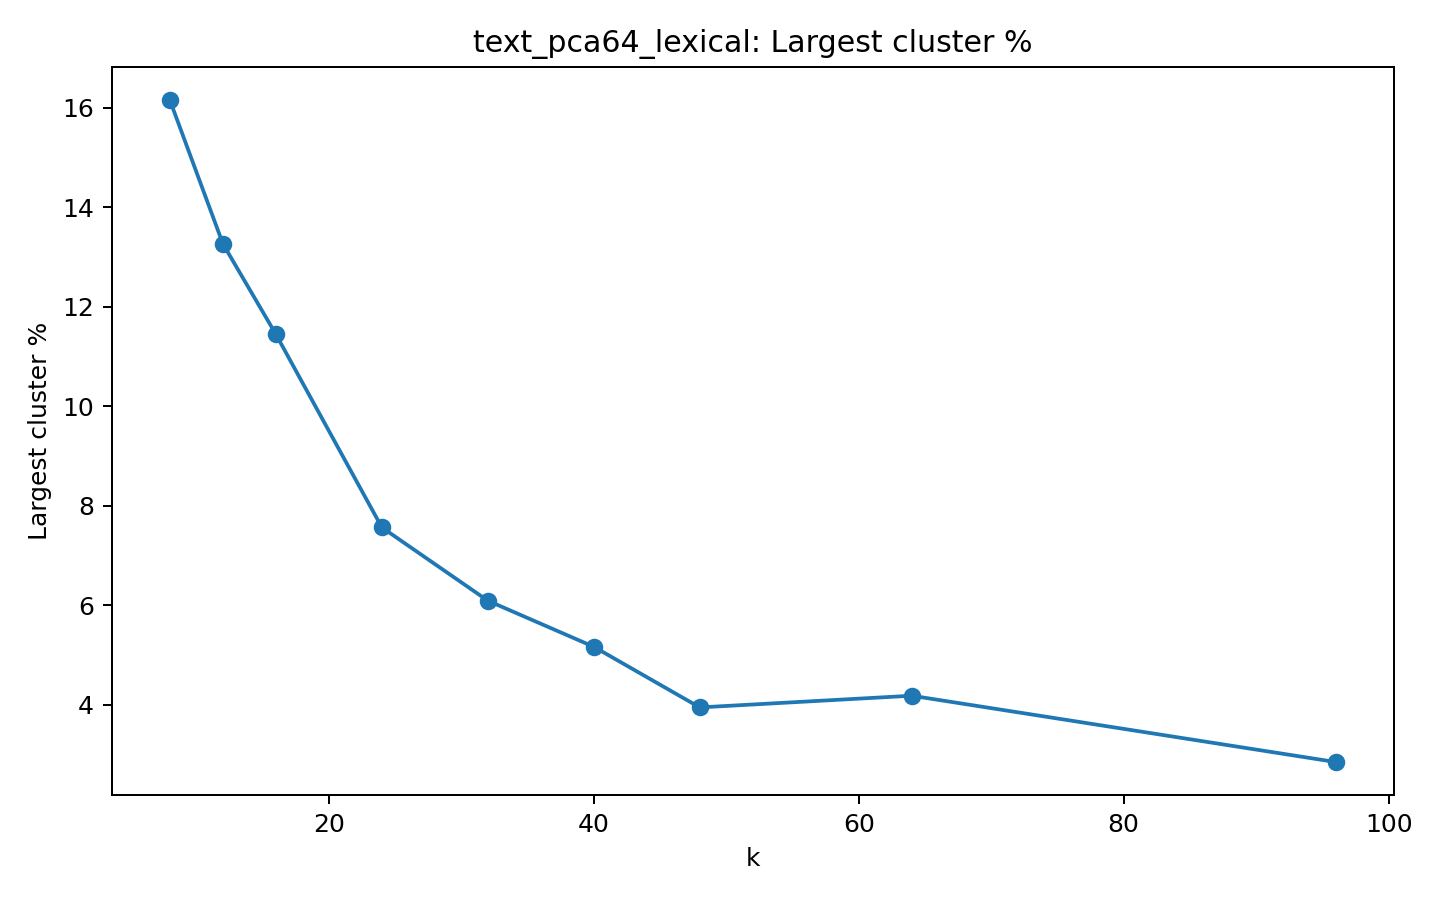
\includegraphics[width=0.82\linewidth]{k_sweep_cluster_balance_text_pca64_lexical.png}
\caption{Cân bằng kích thước cụm theo \(k\) cho \model{text_pca64_lexical}.}
\label{fig:k-balance}
\end{figure}

\begin{figure}[H]
\centering
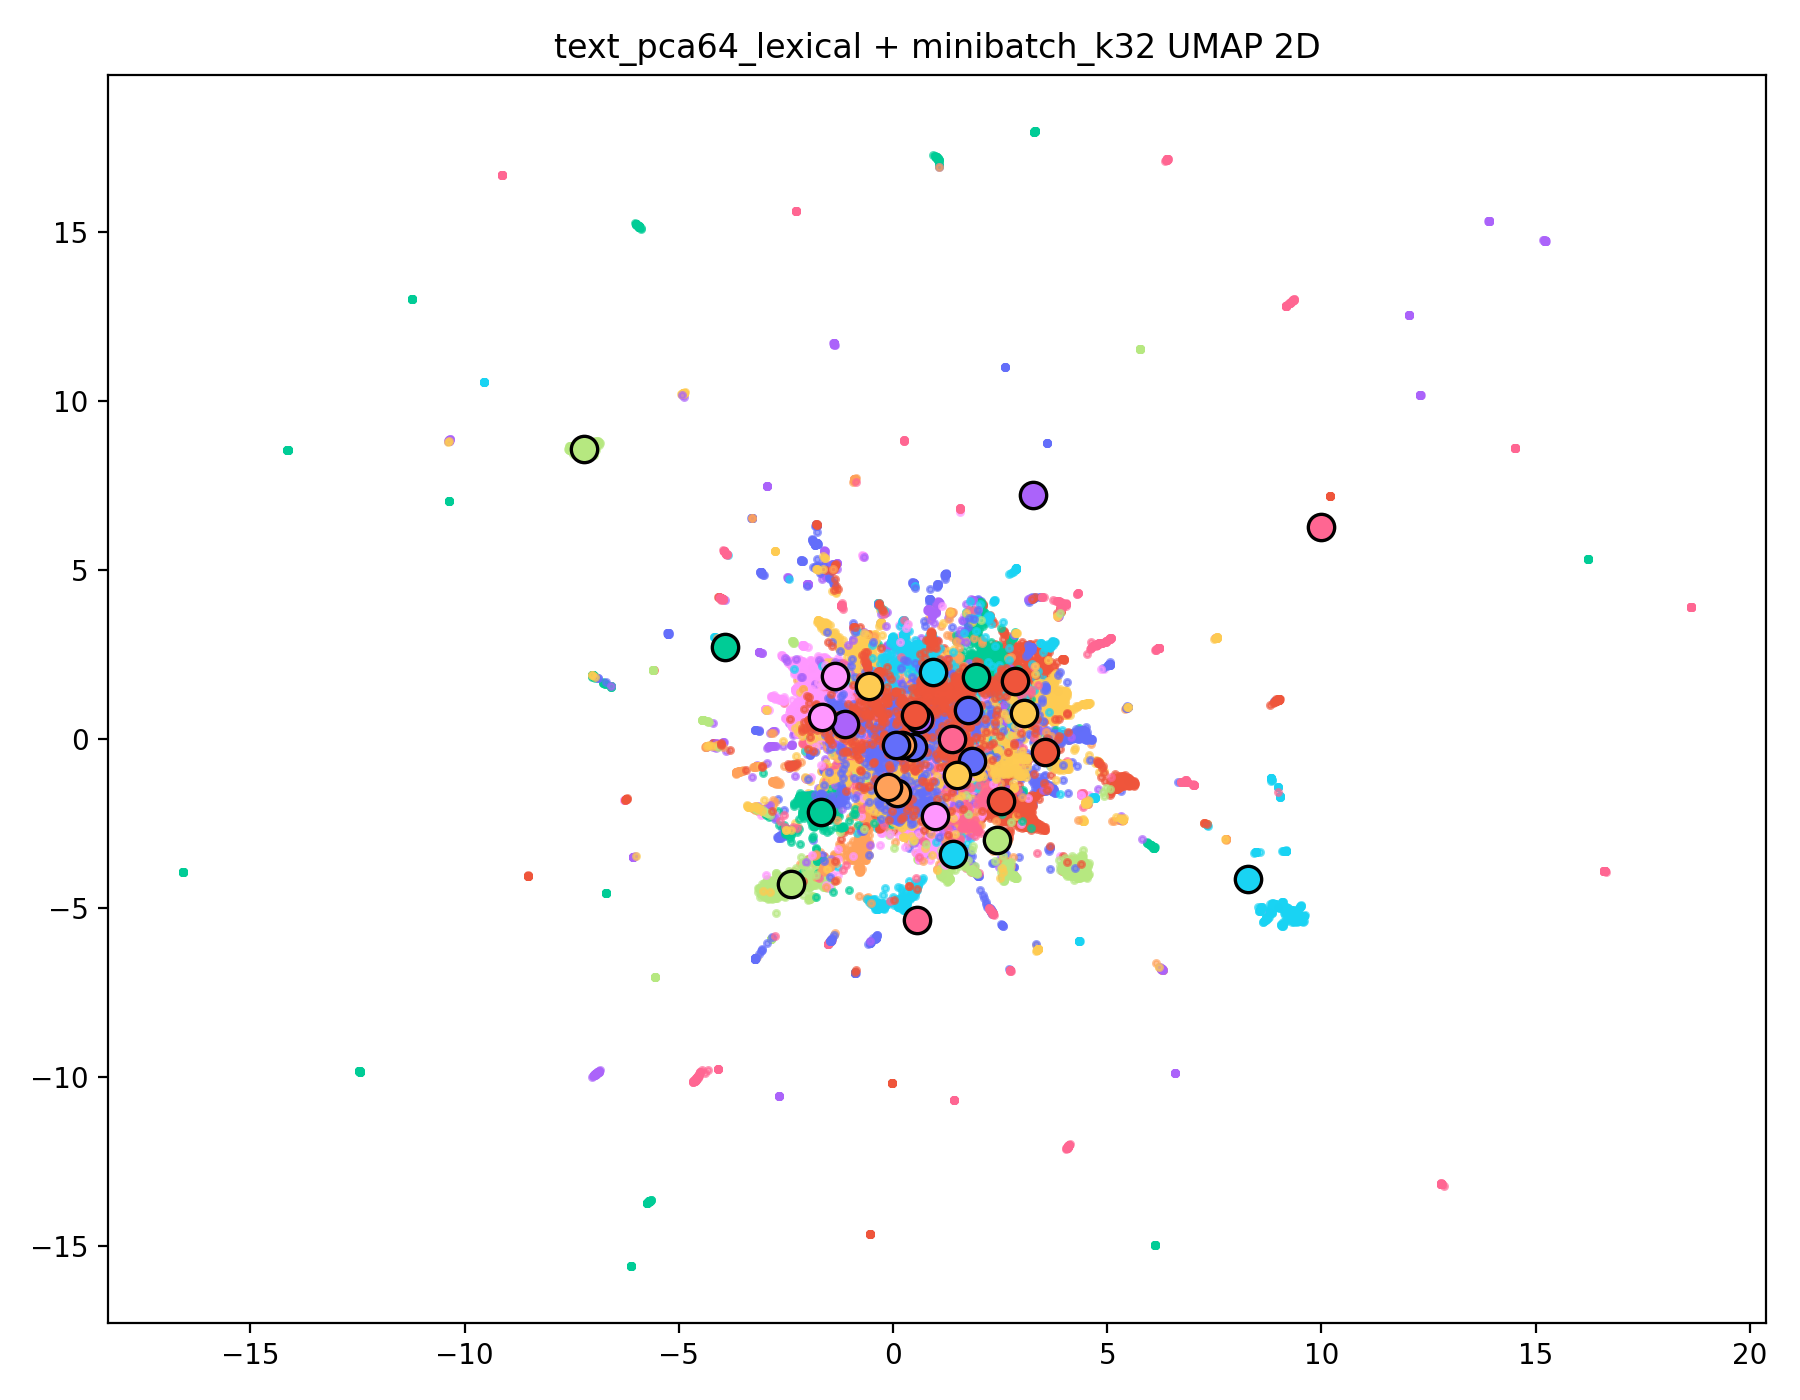
\includegraphics[width=0.82\linewidth]{selected_minibatch_umap_2d.png}
\caption{Trực quan \algo{UMAP} 2D cho mô hình MiniBatch được phân tích sâu. Hình này chỉ dùng như artifact chẩn đoán.}
\label{fig:selected-umap}
\end{figure}

\section{Thảo luận}

Kết quả cho thấy lexical multi-feature nhẹ có thể cải thiện \algo{MiniBatchKMeans} khi \(k\) được chọn cẩn thận. Tuy nhiên, metadata-heavy fusion có thể làm cụm bị chi phối bởi publisher hoặc stock, và \(k\) quá lớn như \model{minibatch_k96} làm tăng fragmentation dù một số metric nội tại trông tốt.

L2 normalization cải thiện DBI và stability trong một số trường hợp, nhưng negative silhouette cao khiến cấu hình \model{text_768_l2} không thay thế được mô hình experimental. PCA64 tuned \algo{HDBSCAN} được chọn cho dense/event detection sau validation full 100k, nhưng kết luận cần kèm caveat rằng một số nhánh HDBSCAN 768D bị timeout.

CLARA true đã được chạy qua \model{sklearn_extra.cluster.CLARA}, không phải fallback. Kết quả tốt nhất chỉ giữ vai trò diagnostic baseline vì silhouette và DBI yếu hơn \algo{MiniBatchKMeans}.

\section{Kết luận}

Báo cáo chọn \model{text_768_original + minibatch_k16} làm conservative full-coverage baseline, \model{text_pca64_lexical + minibatch_k40} làm selected experimental full-coverage model, và \model{text_pca64_only + HDBSCAN(min_cluster_size=30, min_samples=20, leaf)} làm event/dense detection model. \model{text_pca64_only + minibatch_k96} được giữ làm high-silhouette risky reference, không phải mô hình cuối.

Hạn chế chính gồm stability chưa quá cao, publisher dominance trong một số cụm, timeout cho HDBSCAN 768D, chưa có nhãn market-response và chưa có tín hiệu multimodal thực sự. Kết luận phù hợp là \algo{MiniBatchKMeans} trên không gian \model{text_pca64_lexical} là lựa chọn thực nghiệm tốt nhất cho phân cụm phủ toàn bộ dữ liệu, trong khi \algo{HDBSCAN} tuned trên \model{text_pca64_only} nên được dùng riêng cho phát hiện cụm dày hoặc cụm dạng sự kiện.

\appendix
\section{Phụ lục}
\label{app:appendix}

\subsection{Mã nguồn và repository}

Mã nguồn của đồ án được lưu tại repository GitHub:

\begin{center}
\href{https://github.com/medneko/Project-II}{\model{https://github.com/medneko/Project-II}}
\end{center}

Repository chứa các script phục vụ tiền xử lý dữ liệu, trích xuất đặc trưng, sinh embedding, chạy phân cụm, tính metric, sinh hình và tổng hợp bảng kết quả. Báo cáo LaTeX nằm trong thư mục \model{report_latex/} và được thiết kế để biên dịch bằng \algo{XeLaTeX} trên Overleaf.

Một số file dữ liệu lớn và artifact trung gian không được đưa trực tiếp vào project LaTeX, ví dụ \model{.npy}, label CSV lớn hoặc các file kết quả trung gian dung lượng cao. Báo cáo chỉ sử dụng các bảng, hình và summary đã được chọn lọc từ quá trình thực nghiệm.

\subsection{Nguồn kết quả sử dụng trong báo cáo}

Các kết quả trong báo cáo được tổng hợp từ hai nguồn chính:

\begin{itemize}
    \item \textbf{Nguồn mã nguồn và README của repository}: mô tả pipeline tổng quát, cách chạy tiền xử lý, sinh embedding, fusion, phân cụm và các nhóm metric đánh giá.
    \item \textbf{Kết quả thực nghiệm đã sinh trong project}: gồm các file summary, CSV, bảng LaTeX và hình trong thư mục \model{report/runs/100k/}.
\end{itemize}

Các file kết quả quan trọng được dùng để viết phần kết quả và thảo luận gồm:

\begin{itemize}
    \item \model{final_model_comparison_updated.csv}
    \item \model{_k_metric_exploration/metrics/k_sweep_summary.csv}
    \item \model{_k_metric_exploration/metrics/k_sweep_stability.csv}
    \item \model{_hdbscan_tuning_compact/metrics/hdbscan_tuning_summary.csv}
    \item \model{_hdbscan_event_validation/metrics/hdbscan_event_validation_summary.csv}
    \item \model{_multifeature/bounded_ablation/metrics/bounded_ablation_summary.csv}
    \item \model{gmm_k16/metrics/results_summary.csv}
    \item \model{clara_k16/metrics/results_summary.csv}
\end{itemize}

Ngoài ra, bảng so sánh mở rộng các thuật toán được sinh từ script:

\begin{center}
\model{scripts/build_extended_algorithm_comparison_100k.py}
\end{center}

Script này chỉ đọc các summary và CSV có sẵn, không chạy lại clustering, không ghi vào thư mục \model{data/} và không chỉnh sửa các thư mục kết quả đã duyệt.

\subsection{Các artifact hỗ trợ báo cáo mở rộng}

Bộ hỗ trợ báo cáo mở rộng gồm các file sau:

\begin{itemize}
    \item \model{report/runs/100k/_final_analysis/metrics/extended_algorithm_comparison.csv}
    \item \model{report/runs/100k/_final_analysis/metrics/extended_algorithm_comparison.md}
    \item \model{report/runs/100k/_final_analysis/tables/extended_algorithm_comparison.tex}
    \item \model{report/runs/100k/_final_analysis/docs/algorithm_family_comments.md}
    \item \model{report/runs/100k/_final_analysis/docs/report_ready_algorithm_comparison.tex}
\end{itemize}

Các hình so sánh mở rộng được sinh trong thư mục:

\begin{center}
\model{report/runs/100k/_final_analysis/charts/algorithm_comparison/}
\end{center}

Các hình chính gồm:

\begin{itemize}
    \item \model{full_coverage_silhouette_comparison.png}
    \item \model{full_coverage_dbi_comparison.png}
    \item \model{model_scatter_silhouette_vs_dbi.png}
    \item \model{event_models_coverage_comparison.png}
    \item \model{event_models_cluster_count_comparison.png}
    \item \model{stability_ari_comparison.png}
    \item \model{metadata_warning_comparison.png}
    \item \model{cluster_balance_largest_cluster_pct.png}
\end{itemize}

\subsection{Bảng so sánh mở rộng các mô hình}

Bảng~\ref{tab:extended_algorithm_comparison} trình bày đầy đủ hơn các mô hình được chọn, các baseline chính và các cấu hình diagnostic/reference không được chọn. Bảng này được đặt ở phụ lục vì số lượng mô hình tương đối lớn; phần kết quả chính chỉ trình bày nhận xét tổng hợp và một số biểu đồ quan trọng.

\begin{table}[htbp]
\centering
\scriptsize
\caption{So sánh mở rộng các mô hình phân cụm trên tập 100k.}
\label{tab:extended_algorithm_comparison}
\begin{tabularx}{\textwidth}{L{0.17\textwidth} L{0.31\textwidth} L{0.24\textwidth} r r r r}
\toprule
Nhóm & Mô hình & Vai trò & Coverage & Số cụm & Sil. & DBI \\
\midrule
full-coverage & \tablemodel{text_768_original + gmm_k8} & Probabilistic baseline & 100.00 & 8 & 0.0733 & 3.0238 \\
full-coverage & \tablemodel{text_pca64_lexical + minibatch_k40} & Selected experimental & 100.00 & 40 & 0.1065 & 3.3463 \\
full-coverage & \tablemodel{text_768_original + minibatch_k16} & Conservative baseline & 100.00 & 16 & 0.0632 & 3.0854 \\
full-coverage & \tablemodel{text_pca64_all_aux_w005 + minibatch_k32} & Low-weight all-aux reference & 100.00 & 32 & 0.0997 & 3.2368 \\
full-coverage & \tablemodel{text_pca64_all_aux_w030 + minibatch_k32} & Heavier metadata reference & 100.00 & 32 & 0.0927 & 3.7908 \\
full-coverage & \tablemodel{text_pca64_lexical_calendar_publisher_stock + minibatch_k32} & Metadata-heavy reference & 100.00 & 32 & 0.0894 & 3.8401 \\
\midrule
event detection & \tablemodel{text_pca64_lexical + hdbscan_mcs30_ms20_leaf} & Lexical compact candidate & 17.99 & 114 & 0.6120 & 0.9944 \\
event detection & \tablemodel{text_pca64_only + hdbscan} & Selected event model & 20.12 & 219 & 0.6086 & 1.0260 \\
event detection & \tablemodel{text_768_original + hdbscan} & Previous event baseline & 20.64 & 105 & 0.5652 & 0.9861 \\
event detection & \tablemodel{text_pca64_only + hdbscan_mcs50_eom_same_sample} & Same-sample PCA64 baseline & 23.20 & 28 & 0.2236 & 1.0837 \\
event detection & \tablemodel{text_pca64_only + hdbscan_mcs50_ms20_eom} & Same-sample mcs50/eom reference & 20.81 & 59 & 0.5544 & 1.2299 \\
\midrule
diagnostic / reference & \tablemodel{text_pca64_lexical_calendar + clara_k16} & Best CLARA true diagnostic & 100.00 & 16 & 0.0334 & 4.3014 \\
diagnostic / reference & \tablemodel{text_768_original + clara_k16} & Direct CLARA reference & 100.00 & 16 & 0.0146 & 4.3889 \\
diagnostic / reference & \tablemodel{text_768_original + gmm_k16} & Direct GMM reference & 100.00 & 16 & 0.0327 & 2.9701 \\
diagnostic / reference & \tablemodel{text_pca64_only + gmm_k16} & Sampled bounded GMM reference & 100.00 & 16 & 0.0373 & 4.1304 \\
diagnostic / reference & \tablemodel{text_pca64_lexical + minibatch_k64} & Fragmentation watch & 100.00 & 64 & 0.1035 & 3.0478 \\
diagnostic / reference & \tablemodel{text_768_original + minibatch_k32} & Higher-k text baseline & 100.00 & 32 & 0.0836 & 3.2289 \\
diagnostic / reference & \tablemodel{text_pca64_lexical + minibatch_k48} & Strong k-sweep reference & 100.00 & 48 & 0.1109 & 3.1345 \\
diagnostic / reference & \tablemodel{text_pca64_lexical + minibatch_k32} & Previous experimental candidate & 100.00 & 32 & 0.1091 & 3.3961 \\
diagnostic / reference & \tablemodel{text_768_l2 + minibatch_k40} & Representation tuning reference & 100.00 & 40 & 0.0804 & 3.2529 \\
diagnostic / reference & \tablemodel{text_pca64_only + minibatch_k96} & Risky high-k reference & 100.00 & 96 & 0.1161 & 2.9968 \\
\bottomrule
\end{tabularx}
\end{table}


\subsection{Mapping giữa README và báo cáo}

README của repository mô tả pipeline tổng quát của dự án, từ tiền xử lý dữ liệu đến phân cụm và đánh giá. Báo cáo hiện tại kế thừa pipeline đó, nhưng được cập nhật theo kết quả thực nghiệm cuối cùng trên tập 100 nghìn dòng.

Một số điểm đã được điều chỉnh so với README giai đoạn đầu:

\begin{itemize}
    \item README ban đầu mô tả mục tiêu theo hướng \textit{đa thể thức}. Báo cáo hiện tại diễn giải thận trọng hơn: dự án chủ yếu là phân cụm trên không gian vector đa đặc trưng, chưa có ảnh, âm thanh hoặc video thực sự.
    \item Một số KPI ban đầu như ngưỡng \metric{silhouette} hoặc \metric{stability} chỉ được xem là mục tiêu kỳ vọng, không phải điều kiện cứng để kết luận mô hình cuối.
    \item Báo cáo không chọn mô hình theo một metric duy nhất. Quyết định mô hình dựa trên tổng hợp \metric{silhouette}, \metric{DBI}, coverage, noise ratio, cluster balance, stability và hậu kiểm metadata.
    \item Các hình \algo{PCA}/\algo{UMAP} chỉ được dùng như trực quan hóa chẩn đoán, không dùng làm bằng chứng chính để chọn mô hình.
\end{itemize}

\subsection{Mapping giữa mô hình và vai trò sử dụng}

Các mô hình chính trong báo cáo được phân vai như sau:

\begin{table}[H]
\centering
\small
\caption{Mapping giữa mô hình và vai trò sử dụng trong báo cáo.}
\label{tab:appendix-model-role-mapping}
\begin{tabularx}{\textwidth}{L{0.42\textwidth} Y}
\toprule
\textbf{Mô hình} & \textbf{Vai trò trong báo cáo} \\
\midrule
\tablemodel{text_768_original + minibatch_k16} & Baseline thận trọng cho phân cụm phủ toàn bộ dữ liệu. \\
\tablemodel{text_pca64_lexical + minibatch_k40} & Mô hình thực nghiệm được chọn cho nhánh full-coverage. \\
\tablemodel{text_pca64_only + HDBSCAN(min_cluster_size=30, min_samples=20, leaf)} & Mô hình phát hiện cụm dày hoặc cụm dạng sự kiện. \\
\tablemodel{text_pca64_only + minibatch_k96} & Cấu hình tham chiếu rủi ro cao, không phải mô hình cuối. \\
\tablemodel{text_768_l2 + minibatch_k40} & Ứng viên representation tuning, không thay thế mô hình cuối. \\
\tablemodel{text_768_original + gmm_k8} & Baseline xác suất để đối chiếu với \algo{MiniBatchKMeans}. \\
\tablemodel{text_pca64_lexical_calendar + clara_k16} & Diagnostic baseline theo hướng medoid-based. \\
\bottomrule
\end{tabularx}
\end{table}

\subsection{Quy trình trực quan hóa PCA/UMAP}

Các hình trực quan hóa \algo{PCA} và \algo{UMAP} được sinh cho mô hình \model{text_pca64_lexical + minibatch_k40}. Ma trận đầu vào là \model{text_pca64_lexical}, gồm 64 chiều biểu diễn ngữ nghĩa sau \algo{PCA} và 13 đặc trưng lexical, tổng cộng 77 chiều.

Gọi ma trận đặc trưng là:

\begin{equation*}
X \in \mathbb{R}^{n \times 77}.
\end{equation*}

Với \algo{PCA}, dữ liệu được ánh xạ sang không gian thấp chiều bằng phép chiếu tuyến tính:

\begin{equation*}
Z_{\mathrm{PCA}} = \mathrm{PCA}(X).
\end{equation*}

Với \algo{UMAP}, dữ liệu được ánh xạ sang không gian thấp chiều bằng phương pháp phi tuyến nhằm bảo toàn tương đối cấu trúc lân cận:

\begin{equation*}
Z_{\mathrm{UMAP}} = \mathrm{UMAP}(X).
\end{equation*}

Trong cả hai trường hợp, màu của điểm dữ liệu được lấy từ nhãn cụm của \algo{MiniBatchKMeans} với \(K=40\). Như vậy, trực quan hóa không chạy lại phân cụm, mà chỉ chiếu dữ liệu xuống 2D hoặc 3D và tô màu theo nhãn đã có.

Do dữ liệu tin tức tài chính có nhiều chủ đề chồng lấn và mô hình được đánh giá trong không gian nhiều chiều, các hình \algo{PCA}/\algo{UMAP} không nhất thiết cho thấy cụm tách biệt rõ ràng. Vì vậy, các hình này chỉ được dùng làm artifact chẩn đoán và demo, không dùng làm tiêu chí chọn mô hình chính.

\subsection{Ghi chú về khả năng tái lập}

Để tái lập kết quả ở mức báo cáo, người đọc cần có các file summary, CSV và hình đã được sinh trong thư mục \model{report/runs/100k/}. Một số bước như sinh embedding, chạy \algo{HDBSCAN} trên không gian 768 chiều hoặc sweep nhiều cấu hình có thể tốn nhiều thời gian và tài nguyên.

Vì vậy, báo cáo ưu tiên sử dụng các kết quả đã sinh và đã kiểm tra thay vì yêu cầu chạy lại toàn bộ pipeline từ đầu. Cách làm này giúp project LaTeX nhẹ hơn, dễ biên dịch hơn và phù hợp với môi trường Overleaf.

\bibliographystyle{plain}
\bibliography{references}
\end{document}
